
\documentclass{article}
\usepackage[utf8]{inputenc}
\usepackage{graphicx}
\usepackage[T1]{fontenc}
\usepackage{lmodern}
\usepackage{listings}
\usepackage[numbers]{natbib} %IEEE
\usepackage{color}
\usepackage{hyperref}
\usepackage{soul}
\usepackage{float}
\usepackage{pgfplotstable}
\usepackage[font=itshape]{quoting}
\usepackage{booktabs}
\usepackage{amsmath}
\usepackage{multicol}
%\usepackage[table,xcdraw]{xcolor}

\usepackage{minted}
\usepackage[a4paper, total={6in, 8in}]{geometry}
\definecolor{dkgreen}{rgb}{0,0.6,0}
\definecolor{gray}{rgb}{0.5,0.5,0.5}
\definecolor{mauve}{rgb}{0.58,0,0.82}
\definecolor{backcolour}{rgb}{0.95,0.95,0.92}
\definecolor{codegreen}{rgb}{0,0.6,0}
% Define a custom style
\lstdefinestyle{myStyle}{
    backgroundcolor=\color{backcolour},   
    commentstyle=\color{codegreen},
    keywordstyle = \bfseries\color{mauve},
    basicstyle=\ttfamily\footnotesize,
    breakatwhitespace=false,         
    breaklines=true,                 
    keepspaces=true,                 
    numbers=left,       
    numbersep=5pt,                  
    showspaces=false,                
    showstringspaces=false,
    showtabs=false,                  
    tabsize=2,
}
\lstset{style=mystyle}

\title{Data Mining \& Machine Learning \\ \large Computer Exercise 8 - Support Vector Machines}
\author{Steinarr Hrafn Höskuldsson}
\date{October 2022}
\newcommand{\mycomment}[1]{}

\begin{document}
\maketitle
\mycomment{
\begin{figure}[h]
    \centering
    \includegraphics[width=0.75\textwidth]{LAB3/Basic1.png}
    \caption{"Switch test" Breadboard set up}
    \label{fig:Switch_test}
\end{figure}

\lstinputlisting[caption=Defining 'ColorMatch' state, label={lst:colormatch}, language=Python, firstline=44, lastline=52]{LAB3/Basic.py}

}
\section*{Section 1.1}
\begin{figure}[H]
    \centering
    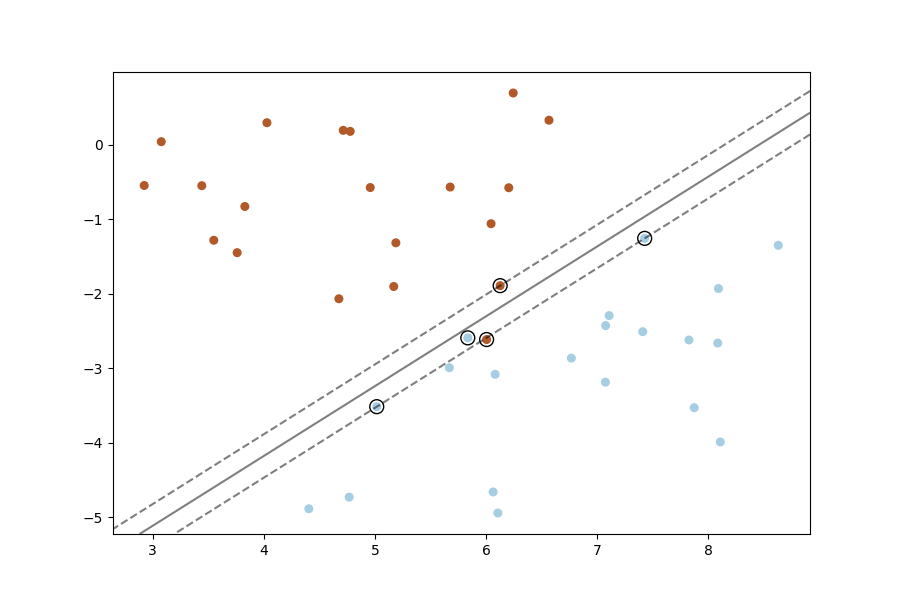
\includegraphics[width=0.75\textwidth]{08_SVM/1_1_1.png}
    \caption{1\_1\_1.png The decision boundary and Support Vector margins for generated data.}
    \label{fig:section11}
\end{figure}

\section*{Section 1.2}
For each class in the support vector machine plotted in Figure \ref{fig:section11} there is one support vector for each of the two classes. Thus the decision boundary is a straight line.

\section*{Section 1.3}
\begin{figure}[H]
    \centering
    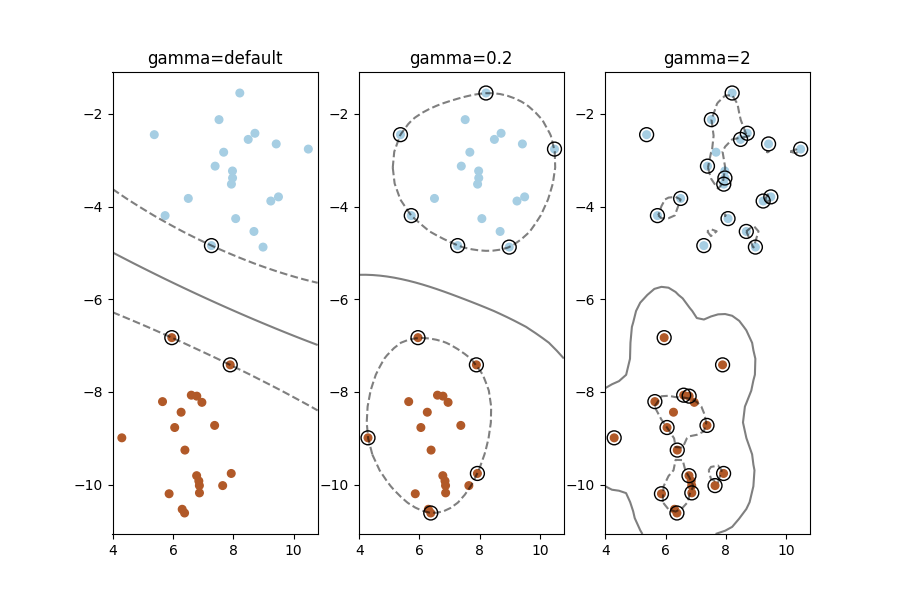
\includegraphics[width=\textwidth]{08_SVM/1_3_1.png}
    \caption{1\_3\_1.png The decision boundary and Support Vector margins for three Support Vector machines that differ only in the value of $gamma$.}
    \label{fig:section13}
\end{figure}

\section*{Section 1.4}
When plotting the decision boundary for different values of gamma as can be seen in Figure \ref{fig:section13} the amount of support vectors were printed:
\begin{verbatim}
For default gamma, number of support vectors is: [1 2]
For gamma=0.2, number of support vectors is: [6 5]
For gamma=2, number of support vectors is: [18 15]
\end{verbatim}

As can be seen on the plots the shape of the decision boundary gets more and more complicated, With default gamma it is a simple curve with a constant curvature, with gamma=0.2 it appears to be a curve with changing curvature and with gamma=2 it is a very complicated shape.

\section*{Section 1.5}
\begin{figure}[H]
    \centering
    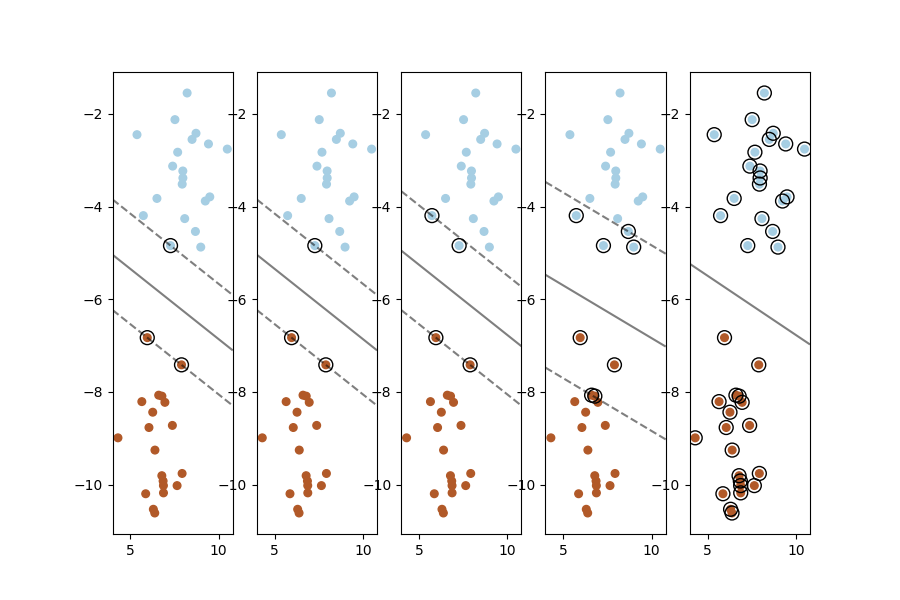
\includegraphics[width=\textwidth]{08_SVM/1_5_1.png}
    \caption{1\_5\_1.png The decision boundary and Support Vector margins for five Support Vector machines that differ only in the value of C}
    \label{fig:section13}
\end{figure}

\section*{}

\begin{verbatim}
For C=1000, number of support vectors is: [1 2]
For C=0.5, number of support vectors is: [1 2]
For C=0.3, number of support vectors is: [2 2]
For C=0.05, number of support vectors is: [4 4]
For C=0.0001, number of support vectors is: [20 20]
\end{verbatim}

\section*{Independent}
\newpage
\section*{Appendix}
\appendix
\section{Code}

\lstinputlisting[ label={lst:colormatch}, language=Python, ]{05_backprop/Steinarr5.py}


\end{document}

